\documentclass[a4paper,10pt]{article}
\usepackage{My_math_package}



\title{MATH620 - Algebraic Number Theory}
\author{Haoran Li}
\date{2018 Fall}

\makeindex[columns=2, title=Index, intoc] % Create the index

\begin{document}\sloppy % reduce overlong words

% Maketitle
\begin{titlepage}
\begin{center}
\vspace*{1cm}
\LARGE
\textbf{MATH621 - Algebraic Number Theory} \\
\vspace{2cm}
\begin{center}
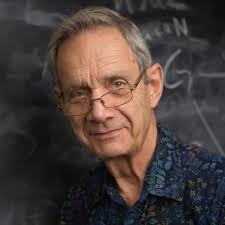
\includegraphics[width=0.5\textwidth]{Pictures/Michael_Artin.jpg}
\end{center}
\vspace{2cm}
\normalsize
Taught by \texttt{Yihang Zhu} \\
Notes taken by \texttt{Haoran Li} \\
2021 Spring \\
\vspace{2cm}
Department of Mathematics\\
University of Maryland\\
\end{center}
\end{titlepage}

\tableofcontents
\newpage

\section{Overview}
\subfile{Overview.tex}
\newpage

\section{Class field theory over $\mathbb Q$}
\subfile{CFT_over_Q.tex}
\newpage

\section{Ramification in $\mathbb Q(\zeta_m)$}
\subfile{Ramification_in_Q(zeta_m).tex}
\newpage

\section{Profinite groups}
\subfile{Profinite_groups.tex}
\newpage

\section{Local fields}
\subfile{Local_fields.tex}
\newpage

\section{Galois theory for local fields}
\subfile{Galois_theory_for_local_fields.tex}
\newpage

\begin{thebibliography}{}



\end{thebibliography}

\printindex

\end{document}